\section{Analog-Digital-Wandler (ADC)}
Der Quantisierungsschritt $q = \frac{V_{refp} - V_{refn}}{2^n}$ wird durch die obere und untere Spannungs bestimmt. Wobei $n$ die Anzahl bits ist. Das Datenwort $D = \frac{V_{in} - V_{refn}}{V_{refp} - V_{ren}}\cdot 2^n$
\subsection{Flash-Wandler (Parallelverfahren)}
Schnell und einfach, aber braucht sehr viel Platz. Runden ist mit verschiedenen Widerständen zuunterst und obest möglich.\\

\textbf{Beispiel} mit $\frac{5}{8}V_{ref}$ was 5 Komperatoren high, und 2 low ergibt. Ausgangswert $5$
\begin{center}
	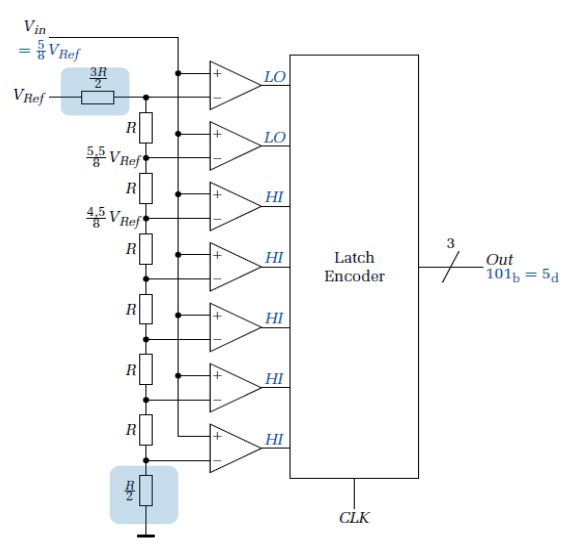
\includegraphics[width=0.6\columnwidth]{Images/adc_parallel}
\end{center}


\subsection{Pipeline-Wandler}
haben gleichen Datendurchsatz wie Flash-Wandler, haben aber Latenz da mehrstufig

\subsection{Successsive Approximation Register (SAR, Wägeverfahren)}
S\&H speichert Eingangssignal wärend Wandlung. mit DAC-Ausgang nährt sich schrittweise dem Eingangssignal an.
\includegraphics[width=\columnwidth]{Images/wägeverfahren_adc}

\subsection{Integrierende Verfahren (Dual Slope, Zählverfahren)}
Integriert bis Komperator schaltet bei $V_{int} = 0$.\\
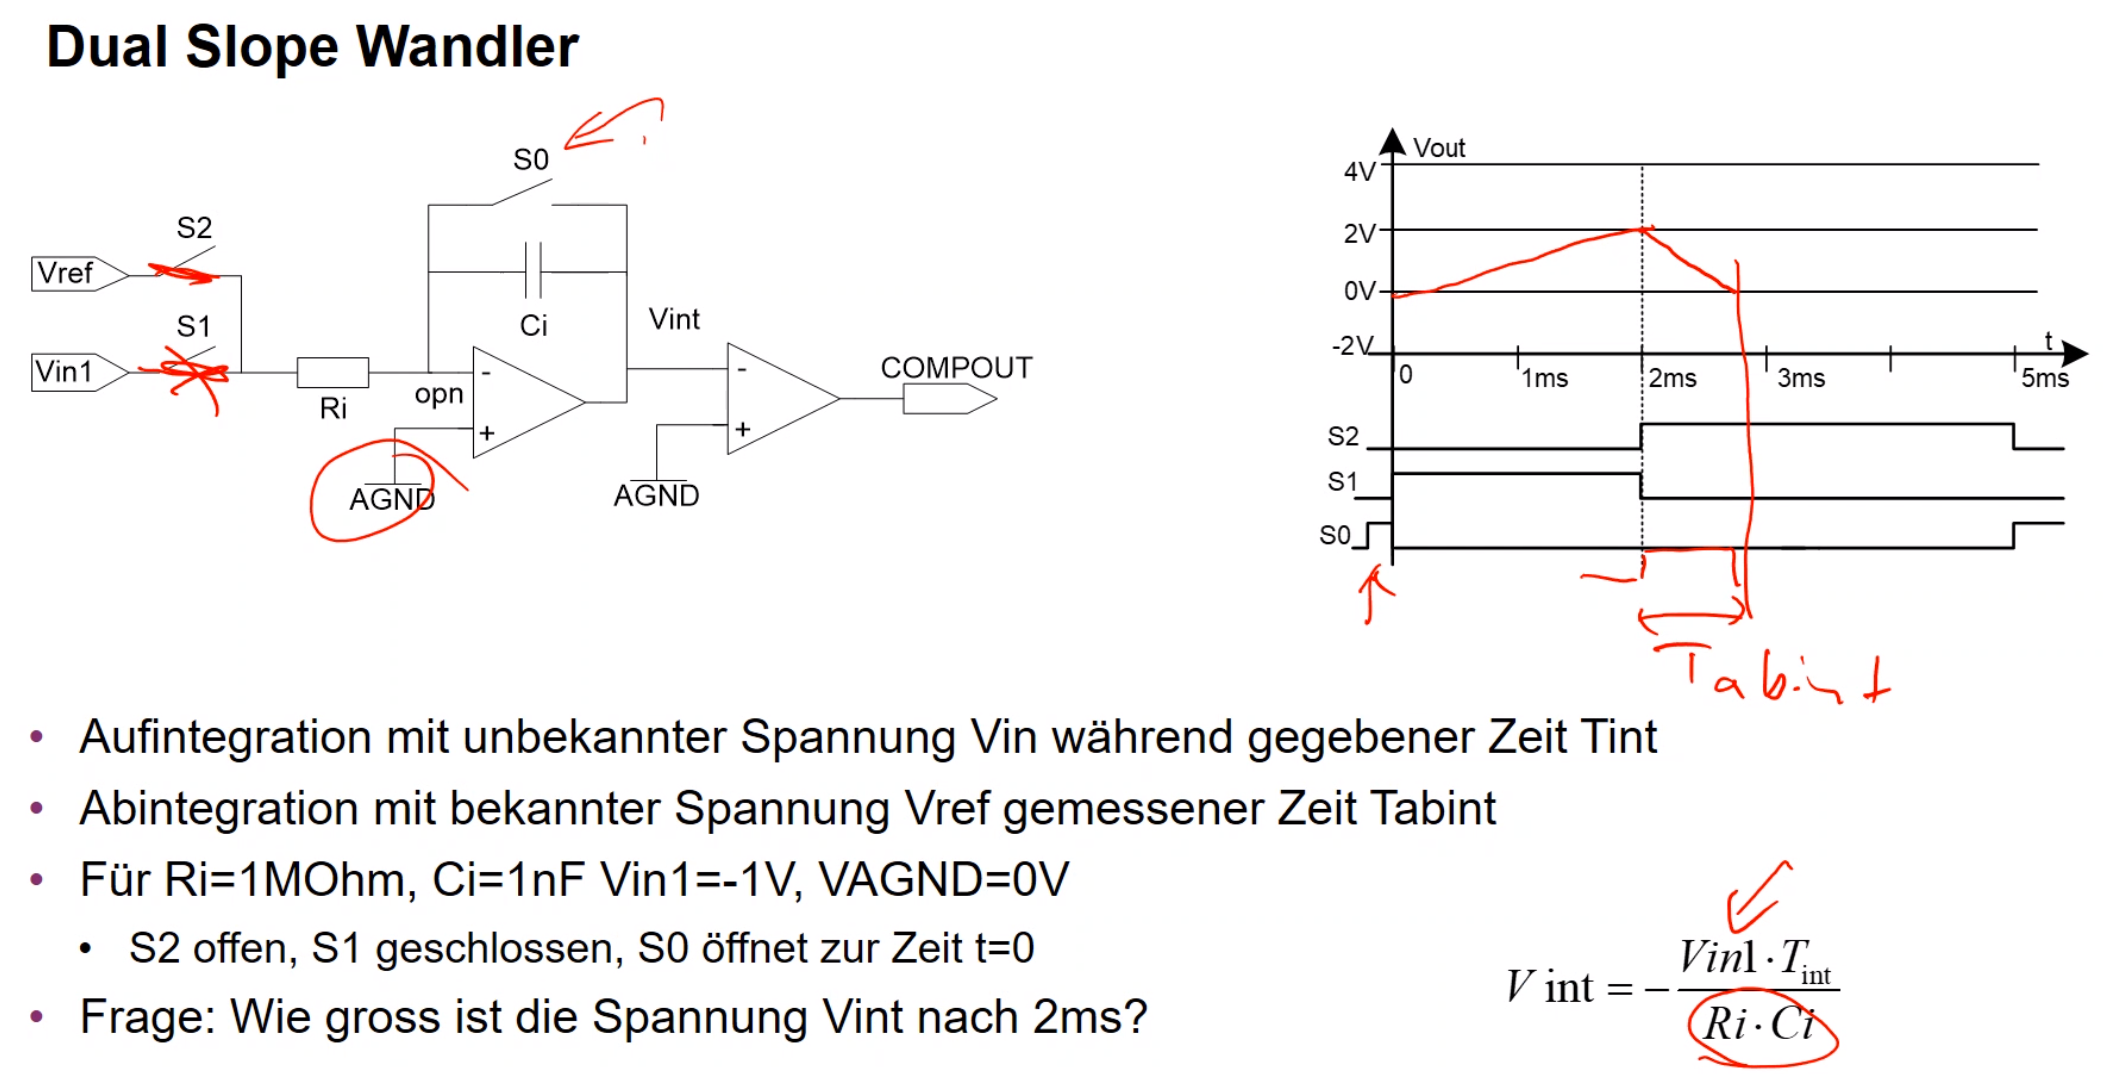
\includegraphics[width=\columnwidth]{Images/dual_slop_adc}
\begin{align*}
	V_{int} &= -\int\limits_{0}^{T_{int}}\frac{1}{R_i \cdot C_i}\cdot V_{in1} dt \\
	V_{int_{max}} &= -\frac{1}{R_i \cdot C_i}V_{in1}\cdot T_{int}\\
	V_{abint}(t) &= V_{int_{max}} - \frac{1}{R_i \cdot C_i}\cdot V_{ref} \cdot t \\
	t_{abint} = -\frac{V_{in1}\cdot T_{int}}{V_{ref}}
\end{align*}

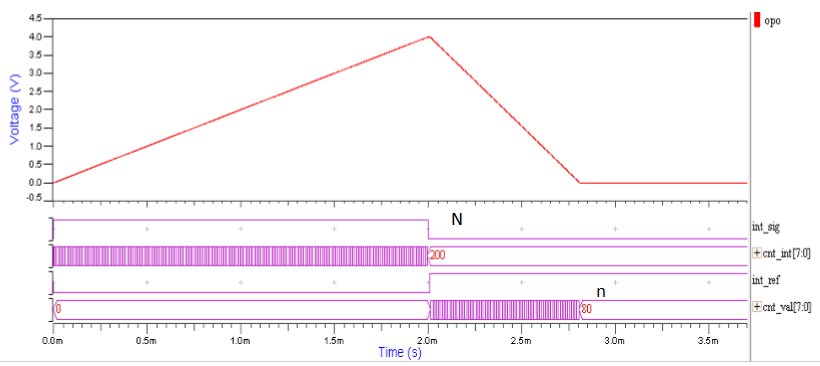
\includegraphics[width=\columnwidth]{Images/dual_slop_adc1}
\[
-\frac{V_{in}}{V_{ref}} = \frac{T_{abint}}{T_{int}} = \frac{n}{N}
\]
\subsection{Fehler}
\begin{enumerate}[nosep]
	\item Gleich wie DAC
	\item Aperturfehler
	\item Alaising
\end{enumerate}